\documentclass[10pt]{article}

% MoML 2026 short paper. Format follows the MoML example style (log_2022.sty, itself
% based on Learning on Graphs 2022): US Letter, single column, Times 10pt, 1.5in side
% margins, 5.5in x 9in text block, non-anonymous. Reproduced here as a self-contained
% preamble so the build has no external style-file dependency.
\usepackage[letterpaper,left=1.5in,right=1.5in,top=1in,bottom=1in]{geometry}
\usepackage{mathptmx}          % Times body + math
\usepackage[T1]{fontenc}
\usepackage[utf8]{inputenc}
\usepackage{amsmath,amssymb}
\usepackage{booktabs}
\usepackage{graphicx}
\usepackage{caption}
\usepackage[dvipsnames]{xcolor}
\usepackage[numbers,sort&compress]{natbib}
\usepackage{titlesec}
\usepackage[hidelinks]{hyperref}

\captionsetup{font=small,labelfont=bf}
\titlespacing*{\section}{0pt}{6pt}{2pt}
\titlespacing*{\subsection}{0pt}{4pt}{1pt}
\titleformat{\section}{\normalfont\large\bfseries}{\thesection}{0.5em}{}
\titleformat{\subsection}{\normalfont\normalsize\bfseries}{\thesubsection}{0.5em}{}
\setlength{\parindent}{0pt}
\setlength{\parskip}{5.0pt}
\newcommand{\alphab}{\ensuremath{\alpha}}

\title{\vspace{-2.2em}\textbf{\large Know When to Fold: Risk-Controlled Abstention for\\
Protein--Ligand Co-Folding under Novelty Shift}}
\author{Rikhin Kavuru\\ \small Independent Researcher \\ \small \texttt{rikhin@virahacks.com}}
\date{}

\begin{document}
\maketitle
\vspace{-2.4em}

\begin{abstract}
\small
Protein--ligand co-folding models (AlphaFold3, Boltz, Chai) report confidence scores that
correlate with pose accuracy, yet a correlation is not a decision rule and it is weakest on
the novel pockets and chemotypes that drug discovery cares about. We build \texttt{foldgate},
a training-free layer that turns frozen co-folding confidence into a risk-controlled
accept/abstain gate with a finite-sample selective-risk guarantee, and we show the guarantee
collapses under training-similarity shift: a marginally compliant gate under-controls error by
about a factor of two on novel strata, and calibrating on familiar targets while deploying on novel
ones violates the guarantee in every run. Measuring reliability drift, the movement of
$P(\text{correct}\mid\text{confidence})$ along a novelty axis, shows the shift is concept shift,
large on structure and near zero on recency. We then prove what that implies. For a threshold on a
frozen score the realized target risk is the covariate-corrected reference plus an accept-region
concept gap that is invariant to any training-free reweighting. So weighted conformal silently
violates its own certificate, level $\alpha$ is unachievable at the operating coverage once the gap
exceeds the remaining slack, and only in-stratum recalibration attains the floor, given stratum
labels. We validate the theorem against a known conditional and on public tabular benchmarks, and
repair coverage with group-conditional calibration and a label-free worst-subpopulation (CVaR/DRO)
certificate under multiplicity control. We then bracket the theorem from both sides. The
impossibility is one-sided, so we certify \emph{danger} label-free instead: cross-model pose
disagreement converts, by triangle inequality against the latent crystal pose, into a valid lower
bound on ensemble risk that runs from $0.01$ on familiar chemotypes to $0.11$ on novel ones. That
escape is narrow, because the floor is blind to consensus error, and the consensus regime it cannot
see covers $64\%$ of the analyzed complexes while the error hidden inside it grows exactly where
risk is highest. On the label side, a per-stratum feasibility map shows the frontier of feasible
coverage decaying to zero on novel strata, so no label budget certifies there, while on the strata
that remain an exact binomial test is the cheapest certifier we find. On a released co-folded virtual screen the pose-confidence signal the layer is calibrated on
enriches actives above docking on the post-2022 novel targets (EF@1\% $9.3$ vs $2.0$), and abstaining
on unreliable poses preserves enrichment that random abstention destroys on $75\%$ of them.
Everything runs on released predictions with no GPU.
\end{abstract}

\section{Introduction}
Co-folding models predict a protein--ligand complex and emit confidence scores (ipTM,
ranking score, PAE). A practitioner who wants to act on a predicted pose needs a decision
rule that carries an error guarantee. Conformal selective prediction supplies one:
accept a pose when its score clears a threshold, abstain otherwise, and certify that the error
rate among accepted poses stays below a target $\alpha$ with high probability~\citep{vovk2005,geifman2017}. The catch is
that this guarantee assumes exchangeability, which breaks precisely where deployment matters,
on ligands and pockets dissimilar to the training set.

We make six contributions, all training-free with respect to the co-folding model and all
computed from released predictions on CPU. (1) We give a finite-sample selective-risk gate
over frozen co-folding confidence and show its guarantee collapses under novelty shift, then
measure \emph{reliability drift} to identify the collapse as concept shift (Sec.~\ref{sec:break}).
(2) We prove an impossibility and a matching achievability result characterizing what a
training-free reweighting of a frozen score can control under concept shift, validated against a
known conditional and on a public non-co-folding benchmark (Sec.~\ref{sec:theory}). (3) Because that
impossibility forbids only certified \emph{upper} bounds, we route around it and certify danger
label-free, converting cross-model pose disagreement into a valid lower bound on ensemble risk, and
we show the escape is structurally narrow and say by how much (Sec.~\ref{sec:danger}). (4) We repair
coverage with group-conditional calibration and a label-free worst-subpopulation CVaR/DRO
certificate, with explicit multiplicity control across the five models (Sec.~\ref{sec:repair}).
(5) We map the price of the repair, showing per stratum where target labels can certify the deployed
rule and where the frontier of certifiable coverage is zero and no budget helps
(Sec.~\ref{sec:cost}). (6) We produce the downstream decision on the pose-confidence signal the gate
is calibrated on: on a released co-folded screen, abstaining on unreliable poses lifts enrichment on
novel targets (Sec.~\ref{sec:screen}). Together these close a bracket: the concept gap cannot be
certified away, cannot be fully exposed label-free, and cannot be bought off with labels where it
matters most.

\section{The gate}\label{sec:method}
We consider a delivered top-1 pose per system with a native confidence $s$ and a binary label
$Y=1$ iff the symmetry-corrected ligand-RMSD is at most $2$\,\AA. The gate accepts when
$s\ge\tau$. We pick the largest accept set (smallest $\tau$) whose selective risk is certified
below $\alpha$ by Learn-then-Test with fixed-sequence testing~\citep{angelopoulos2021ltt}, testing
each $H_0(\tau)\!:\,P(\text{error}\mid s\ge\tau)\ge\alpha$ with an exact binomial tail along a
pre-specified coverage grid; this gives $P(\text{selective risk}\le\alpha)\ge 1-\delta$,
finite-sample and distribution-free. We optionally replace $s$ with a calibration-only combined
score, a shallow gradient-boosted map from cheap per-prediction features (confidence, interface
ipTM, ensemble spread, cross-model agreement, ligand descriptors) to $P(\text{correct})$; the
co-folding model is never retrained, and novelty is excluded from the score and enters only in
calibration. We evaluate five models
(AF3~\citep{af3}, Boltz-1, Boltz-1x, Chai-1, Protenix~\citep{boltz}) on Runs N' Poses~\citep{rnp}, 13{,}535 delivered
poses, at $\alpha=0.20$, $\delta=0.10$.

\section{The exchangeability break and its mechanism}\label{sec:break}
\textbf{The break.} We stratify targets by training-set structural and chemical similarity into
$S_0$ (familiar) through $S_4$ (no analog). A single global threshold hides severe per-stratum
under-coverage: for AF3 the marginal realized risk of $0.177$ masks $0.375$ on $S_3$ and $0.427$
on $S_4$. The operational failure is starker. When we calibrate the gate on familiar targets and
deploy it on the novel region, the realized error is $0.55$ while the target is $0.20$, and the
finite-sample guarantee holds in $0$ of $100$ resampled runs across all models. Marginal
validity is not enough, which is the whole point.

\textbf{Why it breaks.} Weighted conformal would fix this if the shift were pure covariate shift,
where the map $P(Y\mid s)$ is stable and only the marginal $P(s)$ moves. We test that assumption
directly by measuring \emph{reliability drift}
$D(\nu)=\sum_{\text{bins}} w\,[\,P(Y\mid s,S_0)-P(Y\mid s,S_\nu)\,]$, the confidence-conditional
correctness gap between the familiar reference and stratum $\nu$. Drift is large and its 90\%
bootstrap interval excludes zero for every model on structural novelty (Protenix reaches $+0.63$
on pocket novelty, Chai $+0.52$); on temporal novelty it is an order of magnitude smaller
($|D|\le0.07$, with only $2$ of $15$ temporal cells statistically resolved). Confidence is
optimistic on novel structure, the signature of concept shift. A signed accept-region decomposition
makes this quantitative: for AF3 on $S_3$ the target risk gap of $0.328$ splits into a concept term
of $0.309$ (90\% CI $[0.27,0.35]$) and a covariate term of $0.018$, which the next section turns
into a theorem.

\section{What a training-free reweighting can and cannot fix}\label{sec:theory}
The decomposition above is an instance of a general fact. Fix the frozen score $s$ and the accept
rule $\{s\ge\tau\}$. Let $\eta_P(x)=P(Y{=}1\mid X{=}x)$ and $\eta_Q$ be the error conditionals on
the calibration law $P$ and the deployment law $Q$, and call a reweighting \emph{training-free} if
its weights are covariate-measurable and use no target labels (density-ratio, classifier, or
KLIEP weights, including the point mass of weighted conformal). Write $R_{\mathrm{ref}}(\tau_c)=
\mathbb{E}_Q[\eta_P\mid s\ge\tau_c]$ for the covariate-corrected reference at coverage $c$ and
$\bar\Delta_c=\mathbb{E}_Q[\eta_Q-\eta_P\mid s\ge\tau_c]$ for the accept-region concept gap.

\begin{quote}\small
\textbf{Theorem (impossibility, informal; App.~\ref{app:proof}).} At fixed coverage $c$ the realized
target selective risk is $R_Q(\tau_c)=R_{\mathrm{ref}}(\tau_c)+\bar\Delta_c$, and $\bar\Delta_c$ is
\emph{invariant} to the choice of training-free weights. Hence (i) the oracle-weighted plug-in
certificate reports $R_{\mathrm{ref}}$ and still under-states the realized risk by $\bar\Delta_c$;
and (ii) level $\alpha$
is unachievable at coverage $c$ by any training-free reweighting whenever
$\bar\Delta_c>\alpha-R_{\mathrm{ref}}(\tau_c)$.
\end{quote}

The proof (App.~\ref{app:proof}) is a tower-property identity: a covariate-measurable weight
recovers only the \emph{source} conditional $\eta_P$ and cannot reach $\eta_Q$, which completes the
covariate-shift boundary of weighted conformal~\citep{tibshirani2019} and specializes the
irreducible term of domain-adaptation lower bounds~\citep{bendavid2010}. Matching achievability:
in-stratum recalibration attains the floor $R_{Q_g}$ given $n_g$ stratum labels, with slack
$O(\sqrt{\log(1/\delta)/n_g})$; pointwise conditional coverage being
impossible~\citep{barber2021limits}, the guarantee is neighborhood-conditional.

\textbf{Validation on a general benchmark.} A synthetic generator with a known $P(Y\mid s,\nu)$
gives ground truth for each claim. With genuine target drift, $R_{\mathrm{ref}}=0.273$ and
$\bar\Delta=0.205$ sum to the realized $R_Q=0.478$, the realized risk is invariant across nine
reweightings (residual $<0.001$), the oracle certificate under-reports by $\bar\Delta$, and above
the crossing no reweighting reaches $\alpha$; in-stratum recalibration controls only with
target-stratum labels, and an error floor above $\alpha$ forces abstention. A shared-label variant
reproduces the decomposition and invariance with a near-zero pooled gap, placing the concept effect
at the worst stratum as in the co-folding break. On public benchmarks
with no co-folding, a single-threshold gate under-controls the worst novelty block, weighted
conformal issues a certificate its realized risk then violates, and group-conditional calibration
certifies control by abstaining on the blocks it cannot cover: on elec2 (worst-block concept gap
$0.36$) the realized worst-block risks are $0.31$, $0.34$, and $0.20$, and on ACS Income (covariate
gap $0.05$) weighted conformal already repairs the worst state ($0.23\to0.20$).

\begin{figure}[t]
\centering
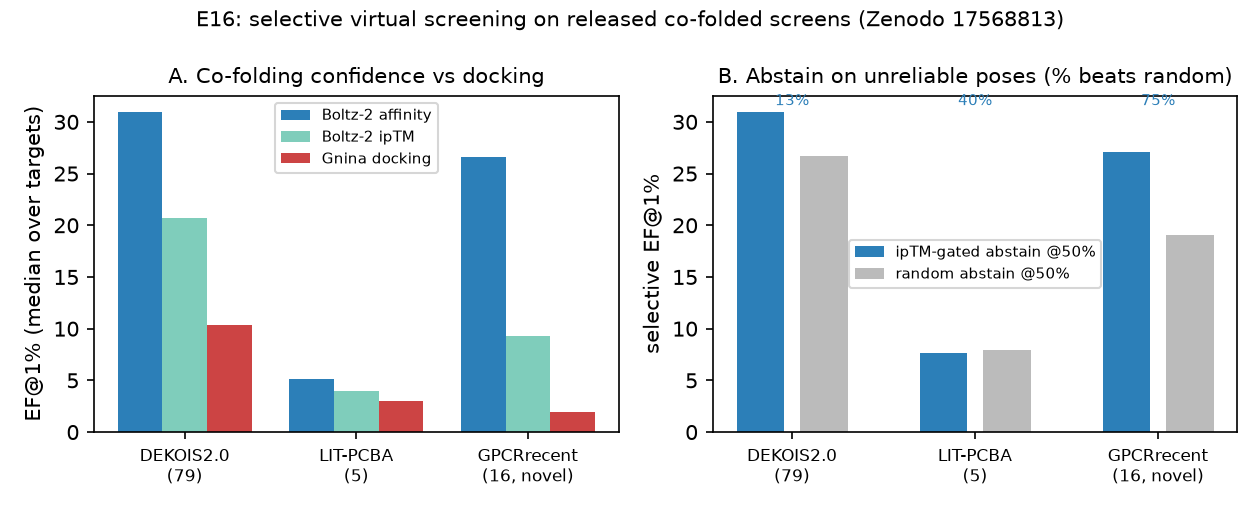
\includegraphics[width=0.66\textwidth]{../results/figures/e16_selective_screening.png}
\caption{Selective virtual screening on released co-folded screens. (A) The pose signal (ipTM) the
layer governs enriches actives above docking, with the ungoverned Boltz-2 affinity head shown for
comparison; the gap is largest on the post-2022 novel GPCR targets. (B) Ranking by the affinity head
and abstaining on low-ipTM poses at $50\%$ coverage preserves enrichment that random abstention
destroys; percentages are the fraction of targets whose selective EF beats the random-abstention
$95$th percentile.}
\label{fig:screen}
\end{figure}

\begin{table}[t]
\centering\small
\caption{Selected results. AURC is out-of-fold under target-grouped (leakage-free)
cross-validation; $m^\star$ is the smallest accepted-mass fraction certified at $\alpha$ by the
label-free CVaR bound. $^{\dagger}$Chai native ranking certifies almost no coverage alone, an honest
limit the combined score recovers.}
\label{tab:results}
\begin{tabular}{lccccc}
\toprule
 & AF3 & Boltz-1 & Boltz-1x & Chai-1 & Protenix \\
\midrule
AURC native $\to$ combined & $.185\!\to\!.118$ & $.234\!\to\!.162$ & $.215\!\to\!.154$ & $.247\!\to\!.146$ & $.281\!\to\!.166$ \\
LOTO realized risk ($\le\!.20$) & $.185$ & $.157$ & $.168$ & $.30^{\dagger}$ & $.191$ \\
reliability drift $D$, pocket $S_3$ & $+.47$ & $+.47$ & $+.47$ & $+.52$ & $+.63$ \\
coverage to certify $m^\star\!\le\!.5$ & $.45$ & $.20$ & $.25$ & $.40$ & $.25$ \\
\bottomrule
\end{tabular}
\end{table}

\section{Certifying danger without labels}\label{sec:danger}
The impossibility is one-sided. What it forbids is a training-free \emph{upper} bound on risk,
because a covariate-measurable weight recovers only $\eta_P$. It places no constraint on a certified
\emph{lower} bound, and the structured output supplies one. Pose correctness is a thresholded
distance, $Y_m=\mathbf 1\{\mathrm{RMSD}(x_m,y^\star)\le\rho\}$ with $\rho=2$\,\AA, so whenever two
frozen models' poses lie more than $2\rho$ apart the triangle inequality forces at least one of them
to be wrong. Disagreement is covariate-measurable, so it adds nothing to the theorem's information
set; what puts it outside the theorem is its direction, since it bounds risk from below, where the
theorem is silent.

We concede the mechanism. That disagreement among frozen models supplies a sound, oracle-free lower
bound on error is already published, for generated code~\citep{incoherence} and, through the
total-variation diameter of credal sets, for classification under shift~\citep{credal}; the pairwise
inequality and its factor one-half are elementary, and wrapping a disagreement indicator in a
one-sided Clopper-Pearson bound is textbook binomial inference. The empirical folklore that pose
agreement filters wrong poses is older still~\citep{consensusdocking}. What is ours is the
conversion of a \emph{continuous} structured output into an error count against a \emph{latent}
target through the $2\rho$ trigger, the $K$-model packing floor, the diverse-versus-consensus
decomposition, and the reconciliation above.

\textbf{One frame, or no theorem.} The triangle inequality relates three points in one metric space,
so the pairwise distance and the label must be measured after the \emph{same} superposition. We
define the pocket once from the crystal ligand, superpose every model's receptor onto the crystal
receptor on those shared C$\alpha$, and recompute both the label and every pairwise distance in that
frozen frame with symmetry-corrected RMSD at \texttt{minimize=False}, which is a genuine quotient
metric under the ligand automorphism group. This step is where the result is won or lost, and it
carries a trap worth reporting. Runs N' Poses ships only the system's receptor chain while a
co-folding model routinely predicts the full assembly, so a chain-ordinal correspondence superposes
onto whichever protomer comes first; for a homodimer the wrong protomer fits the backbone just as
well, leaving the residual $\varepsilon$ small while the ligand is carried tens of \AA ngstr\"om into
the other site. Neither $\varepsilon$ nor the triangle-inequality check sees this, since a displaced
pose is far from everything and satisfies the inequality vacuously: the check passed at $0/13{,}146$
violations while $21\%$ of recomputed distances sat more than $5$\,\AA\ from the shipped value and
$15\%$ of binary labels flipped. Only an external comparison exposes it. Restricting to
instances with a single-chain receptor and an unambiguous ligand copy ($6{,}223$ of $13{,}618$)
raises agreement with the shipped BiSyRMSD label from Spearman $0.620$ to $0.995$ (Pearson $0.999$,
correctness calls agreeing $99.4\%$, $0.1\%$ off by more than $5$\,\AA). The exclusion is a property
of the system rather than the model, since the models never disagree on predicted chain count
($0/2303$) and per-model survival is uniform ($42$--$51\%$), so cross-model comparison stays fair.
The kept subset is not a random half of the benchmark, and we report its composition rather than
correct it: it is slightly more novel (mean ligand similarity $0.452$ against $0.500$) and slightly
less accurate ($0.651$ against $0.672$) than the excluded half, so the floors below describe the
single-chain half of Runs N' Poses. $1{,}115$ instances retain all $K{=}5$ models, and that is the
sample every number below runs on. Recovering the excluded half needs a quotient by the receptor
symmetry group, which we leave to future work: resolving the mapping per instance against the
crystal ligand would put a label inside a statistic that must stay label-free.

\textbf{Three floors, each with the tool its estimand admits.} For one pre-registered pair
(AF3 and Chai-1, fixed on the architectural argument rather than on measured disagreement),
$R_{\max}\ge\tfrac12 p_L$ with $p_L$ an exact one-sided Clopper-Pearson bound. For the any-pair
statistic the constant is $1/K$ and not $\tfrac12$, since one model erring away from $K-1$ correct
poses fires the statistic while $R_{\max}=1/K$. The headline is the packing floor: correct poses lie
within $\rho$ of $y^\star$, hence within $2\rho$ of each other, hence carry no edge in the graph $G$
joining poses more than $2\rho$ apart, so they form an independent set and
$\bar R\ge 1-\mathbb{E}[\alpha(G)\mid A]/K$. Here $\alpha(G)/K$ is a bounded mean rather than a
binomial proportion, so Clopper-Pearson is invalid and we use a betting upper
bound~\citep{waudbysmith2024betting}. We keep it because it is variance-adaptive and never worse on
average, not because it buys much: measured against Hoeffding-Bentkus on these cells it is tighter
in $61\%$ of them for a median gain of only $0.006$ of floor, and at the accept counts below $50$
that the novel strata leave the median gain is $0$ and Hoeffding-Bentkus is sometimes tighter.
Because disagreement is symmetric it cannot assign blame, so every floor is stated for the ensemble
mean or the worst model and never for the deployed one. That is a real limit rather than a
conservative choice: if the deployed model were correct everywhere on $A$ while two others erred in
mutually $>2\rho$ directions, the statistic would fire at full strength while the deployed model's
risk was exactly $0$.

\textbf{Valid, and narrow by construction} (Fig.~\ref{fig:d1d2}A,B). The floors never exceed the
realized quantity they bound ($0/386$ cells). That follows from the construction rather than testing the $\delta$ level,
since the pointwise inequality already forces the empirical floor under the empirical risk on the
same sample; what $\delta$ buys is the step from the sample to the population, which no finite check
can exhibit. The floors are not vacuous: marginally the packing floor certifies $\bar R\ge0.124$
against a realized $0.348$. They track novelty, which is the point. For AF3 at $50\%$ coverage on
the ligand axis the certified floor runs $0.010$ on $S_0$ to $0.109$ on $S_3$ while realized
$\bar R$ runs $0.090$ to $0.320$, so a caller with no labels at all learns that ensemble risk on
novel chemotypes is bounded away from zero. The exception is instructive and we state it: on $S_4$,
the no-analog stratum this paper treats as the sharpest extrapolation test, the floor collapses to
$0.000$ for all five models, while realized $\bar R$ runs from $0.000$ to $0.455$ on samples of $1$
to $11$ complexes (AF3: $0.455$ on $n=11$). The certificate is vacuous exactly where the question is
hardest, and the stratum is too thin at this coverage to say more than that.

What the floor does \emph{not} do is expose the theorem's blind spot: it exceeds a bootstrap
$(1-\delta)$ upper bound on $\bar R_{\mathrm{ref}}$ (a percentile interval, asymptotic, unlike the
finite-sample floor it is compared against) in $1$ of $124$ cells at per-cell level $0.80$, which no
family-wise correction survives, so we report it as null. The reason is measured rather than
assumed, and it is structural. The floor is blind to consensus error: when all $K$ models share one
wrong mode, $G$ has no edges, $\alpha(G)=K$, and the floor reads exactly $0$. Over the $1{,}115$
analyzed complexes, consensus covers $64\%$ and carries risk $0.152$ against $0.698$ on the diverse
remainder. Conditioning on AF3's accept region at $50\%$ coverage along the ligand axis, the
consensus rate falls from $0.92$ on $S_0$ to $0.60$ on $S_3$ while the risk \emph{inside} consensus
rises from $0.063$ to $0.200$. The models that still agree are increasingly agreeing on a wrong
mode, so the error the floor cannot see, the consensus rate times the risk inside it, grows from
$0.058$ to $0.120$ even as the consensus mass itself shrinks. Label-free danger certification is
therefore real and valid, and it is structurally too weak to audit the concept gap it is aimed at.
The size of that shortfall is what we contribute.

\begin{figure}[t]
\centering
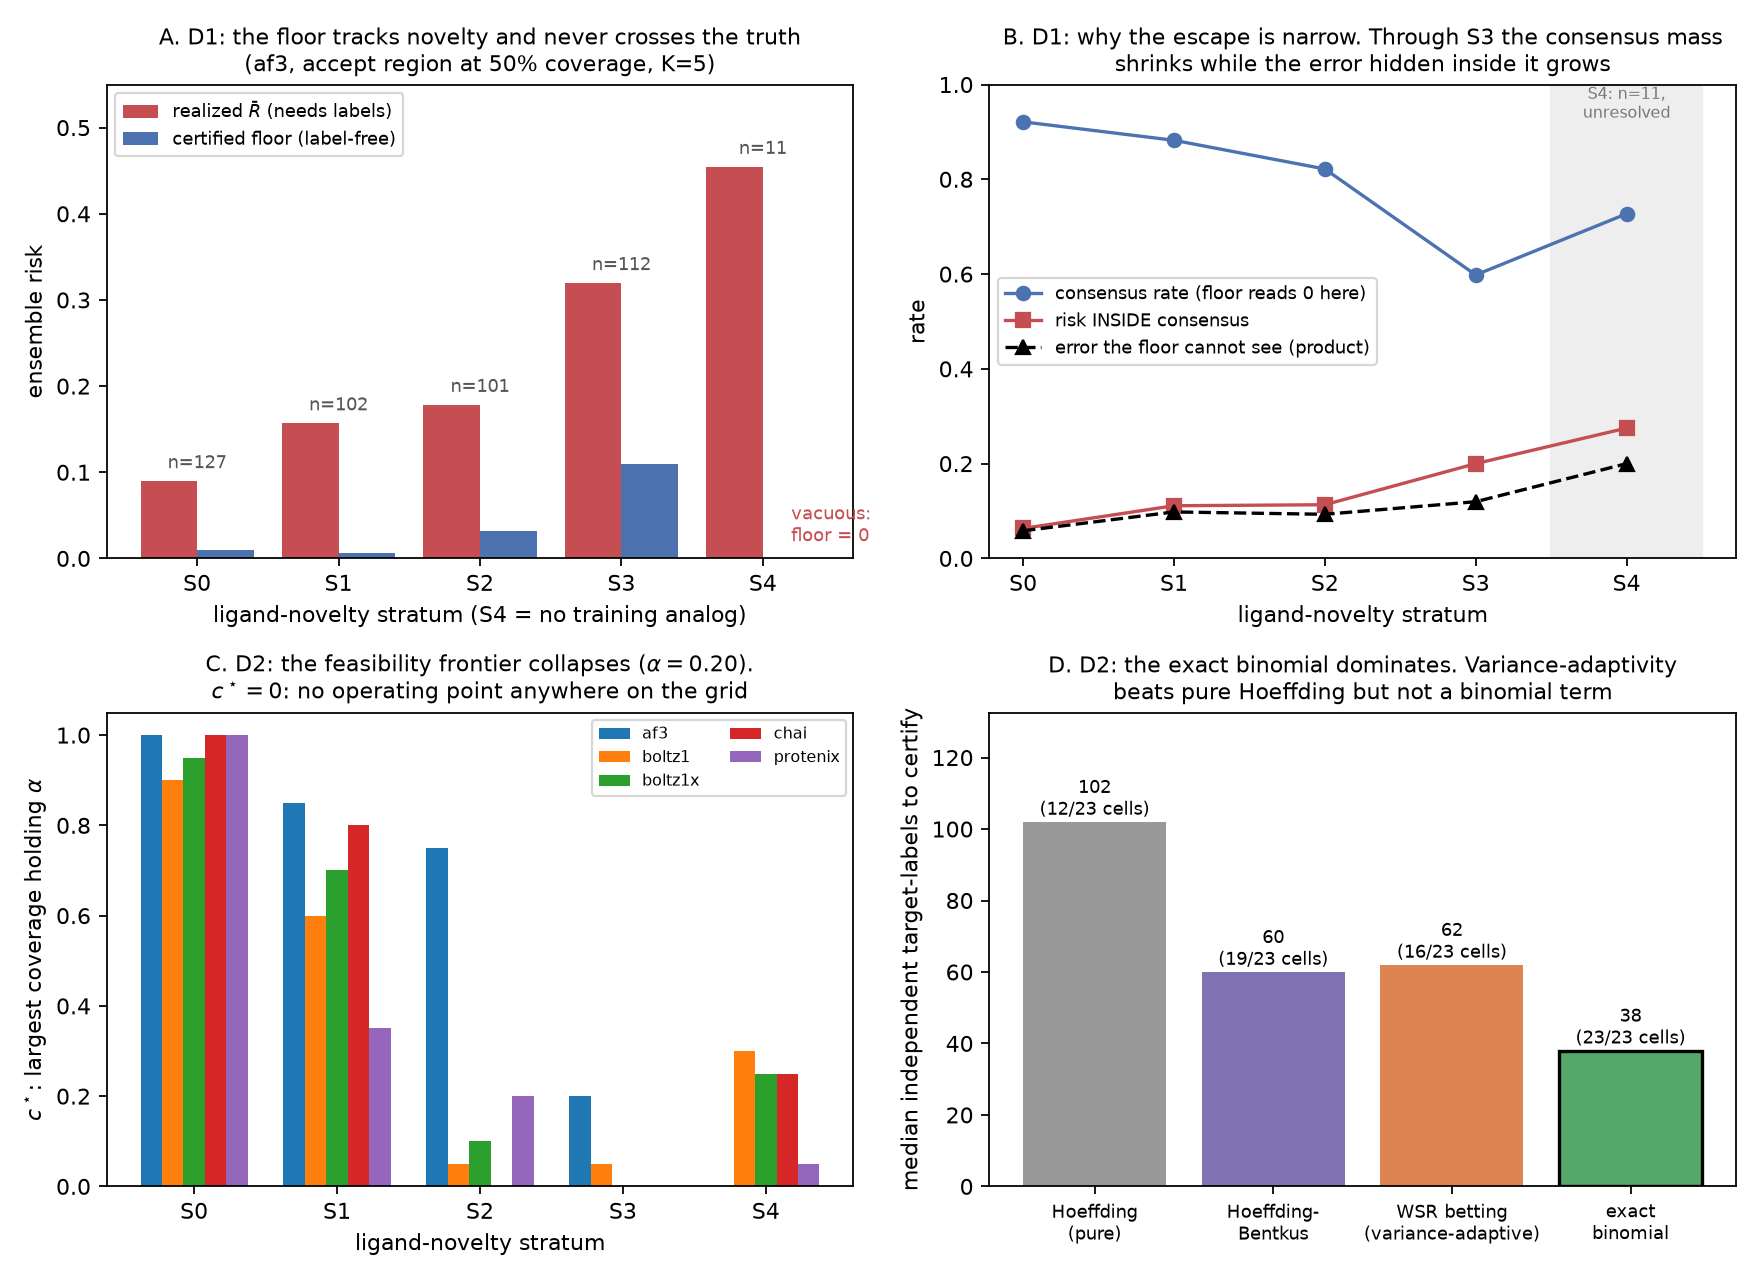
\includegraphics[width=0.92\textwidth]{../results/figures/d1_d2_summary.png}
\caption{The bracket, measured. (A) The label-free disagreement floor tracks novelty and stays under
the realized ensemble risk it bounds, and goes vacuous on the no-analog stratum $S_4$ ($n=11$).
(B) Why the escape is narrow: through $S_3$ the consensus mass the floor cannot see shrinks while
the risk inside it rises, so the hidden error (their product) grows; $S_4$ is unresolved at $n=11$.
(C) The D2 feasibility frontier $c^\star$, the largest source coverage at which the deployed rule
still holds $\alpha=0.20$; zero means no operating point anywhere on the swept grid.
(D) On the cells that remain feasible, the exact binomial certifies with the fewest target-labels
and is the only certifier that fires on all of them; variance-adaptive betting beats \emph{pure}
Hoeffding but not a binomial term.}
\label{fig:d1d2}
\end{figure}

\section{Repairing the guarantee}\label{sec:repair}
\textbf{Group-conditional calibration} keys a separate threshold per novelty stratum, restoring
per-stratum control at an honest coverage cost (with the combined score AF3 accepts $52\%$ of $S_1$
and $39\%$ of $S_2$ at risk $\le\alpha$, against $8\%$ and $12\%$ natively). It needs stratum
labels, which Runs N' Poses ships.

\textbf{A label-free worst-subpopulation certificate.} When the novel subpopulation is unnamed,
we control the conditional value-at-risk of the accepted loss. For the binary label,
$\mathrm{CVaR}_\beta=\min(1,r/(1-\beta))$ with accepted error rate $r$, so a finite-sample upper
bound on $r$~\citep{bates2021rcps} certifies $\mathrm{CVaR}_\beta\le\alpha$ for every $\beta$ at once
\citep{snell2022qrc}. By CVaR--DRO duality this certifies that every accepted subpopulation of
mass at least $m^\star=1-\beta^\star$ has error $\le\alpha$, with no stratum labels and no
importance weights. The combined score certifies $m^\star\le 0.5$ (every half-subpopulation) at
$20$--$45\%$ coverage where the native score often certifies nothing, and is largely vacuous on
deploy-to-novel ($m^\star\!\to\!1$ for most models), which we report. The same certificate reparameterizes to a chi-square
robustness radius $\rho^\star$~\citep{cauchois2024}, and a Bonferroni $\delta/K$ correction yields
one certificate jointly across all five models (at $20\%$ coverage, $m^\star=0.52$ and
$\rho^\star=0.10$ for every model at once).

\textbf{Multiplicity across models.} Joint certificate claims (the gate, leave-one-target-out
validity, the CVaR/DRO bounds) take a Bonferroni union bound at $\delta/K=0.02$; the joint
leave-one-target-out gate then holds for AF3, Boltz-1, and Boltz-1x with real coverage while Chai and
Protenix satisfy it only by abstaining. ``For every model'' significance conjunctions are
intersection-union tests, valid without penalty. The $55$-cell drift grid uses a Romano-Wolf
step-down bootstrap~\citep{romanowolf2005} at family-wise $0.10$; $42$ cells survive, all structural
ones among them, while the temporal cells fail a $0.05$-margin equivalence test, leaving only the
temporal-versus-structural magnitude contrast supported.

\textbf{Weighted conformal serves as a label-free complement} that abstains on real novel data
(Sec.~\ref{sec:theory}), so group-conditional calibration stays the operative guarantee. A
training-free surrogate that keys the gate on the model's own ensemble disagreement recovers control
on moderate novelty but stays a weak proxy on the extreme.

\section{Where labels certify, and where nothing does}\label{sec:cost}
If a label-free certificate cannot see the concept gap and a label-free danger floor is too weak to
expose it, the remaining question is what target labels buy and where. Fix the deployed rule
$\{s\ge\tau\}$ and write the certification margin $m_g=\alpha-R_{Q,g}(\tau)$. Its sign is the whole
map. Where $m_g>0$ the rule really does hold $\alpha$ on stratum $g$, labels can certify it, and the
budget is governed by $m_g$~\citep{csa,ppi}. Where $m_g\le0$ the rule genuinely violates $\alpha$,
and no certificate, label-free or label-fed, can certify a false statement; the only honest action
is to abstain or drop coverage. That is the impossibility regime seen from the label side.

\textbf{The query unit is the target.} Runs N' Poses ships several rows per system when a system has
several ligand instances, and losses cluster hard by target, so pooling them as independent draws is
anti-conservative and silently changes the estimand. We reduce to one delivered pose per
(system, model), which leaves $12{,}125$ independent target-labels over $2{,}425$ systems, and report
every budget in those units.

\textbf{A frontier, not an operating point.} Part (ii) of the theorem (App.~\ref{app:proof}) is
pinned at a fixed coverage and deliberately does not claim $\alpha$ is unreachable at lower
coverage, which would need $R_Q$
monotone in coverage. Reporting one calibrator's threshold would hide that question and would make
the map an artifact: at our default $\alpha=0.20$ the familiar stratum's own risk is $0.13$, already
below $\alpha$, so Learn-then-Test certifies the whole set and the gate degenerates to accepting
everything ($\tau=0.237$ for AF3, coverage $1.00$ on every stratum); and for Chai-1, whose top-ranked
poses contain early errors, fixed-sequence testing rejects its first hypothesis and returns no
threshold at all. Neither degeneracy is a fact about co-folding. So we sweep the rule over source
coverages and report, per stratum, the largest coverage at which it still holds $\alpha$,
$c^\star_g(\alpha)=\max\{c: R_{Q,g}(\tau(c))\le\alpha\}$, calibrating $\tau$ on a held-out half of
the familiar stratum and deploying it frozen.

The frontier decays with novelty through $S_3$ and then vanishes on the strata that matter
(Fig.~\ref{fig:d1d2}C). For AF3
on the ligand axis at $\alpha=0.20$, $c^\star$ runs $1.00,\,0.85,\,0.75,\,0.20,\,0.00$ across $S_0$
to $S_4$; tightening to $\alpha=0.10$ collapses it to $0.65,\,0.40,\,0.10,\,0.00,\,0.00$. The decay
is not monotone at $S_4$, which exceeds $S_3$ in $8$ of the $10$ model-axis cells at both levels:
that is the no-analog bin at $n\approx60$ per model, and its intervals are wide enough that we read
the trend through $S_3$ and report $S_4$ as unresolved. Across models and both novelty axes, $39$ of $50$ strata admit an
operating point at $\alpha=0.20$ and $11$ admit none anywhere on the grid, worsening to $33$ and
$17$ at $\alpha=0.10$. That count is an oracle one, computed from the realized risk with every label
revealed; the honest number a caller could stand behind is smaller, $23$ of the $39$ at
$\alpha=0.20$ and only $3$ of the $33$ at $\alpha=0.10$, where the labels in hand actually certify
the frontier they mark.

A frontier of $0.00$ is the sharper statement: on those strata the frozen score has no operating
point anywhere on the swept grid, which runs down to $5\%$ source coverage, and below that the
accepted set falls under $20$ targets and nothing is resolvable. The claim also survives the
sampling noise on $19$ of the $28$ zero-frontier strata pooled across both levels ($11$ at
$\alpha=0.20$ and $17$ at $\alpha=0.10$), where the exact Clopper-Pearson lower bound
on $R_{Q,g}$ exceeds $\alpha$ at every coverage that leaves enough accepted targets to measure. Even
bounded this way it is stronger than the coverage-pinned theorem, which speaks only at the deployed
coverage, and it is an empirical finding rather than a corollary of it. The deployed view is starker
still. The AF3 rule that Learn-then-Test certifies at $\alpha=0.20$ on familiar targets realizes risk
$0.538$ on $S_3$, a margin of $-0.338$, so the certificate is not merely loose but inverted.

\textbf{What it costs where it is feasible, and a win that does not exist.} On each feasible cell we
hide the labels, reveal one independent target-label at a time in random order, and record the
budget at which each certificate first fires. On the $23$ cells that carry a budget curve (feasible
at a fixed $50\%$ source coverage, $18$ at $\alpha=0.20$ and $5$ at $\alpha=0.10$, a different set
from the label-certified strata above), the \emph{exact binomial} test is the only certifier that
fires in a majority of reveal orders on every one, at a median first-firing budget of $38$
target-labels, against $60$ for Hoeffding-Bentkus ($19/23$ cells), $62$ for a variance-adaptive WSR
betting sequence ($16/23$), and $102$ for pure Hoeffding ($12/23$).

We had expected empirical-Bernstein variance-adaptivity to be the robust saving at the small
accepted error rates these cells show ($R_Q=0.06$ to $0.18$), and it is not: the exact binomial is
cheaper than WSR in $16$ of the $16$ cells where both fire. The reason is structural. The count is a
sufficient statistic for a Bernoulli mean and the exact binomial tail is its exact inversion, so
every fixed-$n$ concentration bound is a relaxation of that tail and none of them is tighter.
Variance-adaptivity is not useless here, and we should say so: WSR is cheaper than \emph{pure}
Hoeffding, which assumes the worst-case variance $\tfrac14$, in $12$ of the $12$ cells where both
fire, at a median of $49$ against $102$. That saving simply closes once the baseline carries a
binomial term, which our Hoeffding-Bentkus certifier already did ($60$ against WSR's $62$), and it
never reaches the exact tail. So the win we planned for was real but aimed at a baseline we had
already beaten.

Two caveats belong with this ranking rather than under it. A fixed-$n$ bound is valid only at a
budget fixed in advance, so reading its first-firing budget off a reveal sequence flatters it,
whereas the WSR sequence is the one construction here that stays valid under optional stopping. The
tilt runs against WSR and WSR loses anyway, so the ordering is conservative; the budgets are not, and
the $38$ is a lower bound on the planned budget a caller could stand behind rather than the price of
a valid certificate. Budgets are also medians over the orders in which a certifier fires, so the two
cells where the binomial fails in $42\%$ and $22\%$ of orders report their successful half. Finally,
the budget grows as the margin shrinks but more slowly than the $\Theta(m_g^{-2})$ rate the theory
predicts~\citep{csa}: a log-log fit over the $23$ cells gives an exponent of $-1.07$ (90\% CI
$[-1.26,-0.91]$). The margin does not determine the budget on its own, since two cells sharing a
margin of $0.025$ and an error rate of $0.075$ cost $164$ and $72$ labels. A
prediction-powered control covariate is likewise a measured null here: the best label-free covariate
reaches median $|\rho|=0.26$, keeping $0.93$ of the variance, and we report it rather than curve-fit
it, since PPI's $(1-\rho^2)$ is asymptotic and its adjusted variable is unbounded, so splicing it
into a finite-sample budget plot would compare two different guarantees.

This is the cost side of the bracket, and it sets the price honestly. Certification is feasible on
the familiar half of the novelty axis, where labels are cheapest and least needed, and it is
infeasible on the novel tail, where the decision matters and where no label budget helps, because
what fails there is the rule and not the estimate of it.

\section{Utility and a downstream decision}\label{sec:screen}
\textbf{Ranking utility, validated without leakage.} The combined score dominates native
confidence on the risk-coverage curve, cutting its area by $28$--$41\%$ (AF3
$0.185\!\to\!0.118$, Protenix $0.281\!\to\!0.166$), about two to three times more poses
retained at a fixed guarantee. Because a target recurs across models, a naive pooled split
leaks $95.1\%$ of test targets into calibration; under target-grouped cross-validation the gate
still holds (AF3 risk $0.185$, $[0.168,0.203]$, $5/5$ folds) and the advantage survives
(Table~\ref{tab:results}).

\textbf{The decision number.} We reuse a released co-folded virtual screen~\citep{shen2026vs}
with per-compound confidence and active/decoy labels for DEKOIS2.0 (79 targets), LIT-PCBA (5),
and GPCRrecent (16 post-2022 novel targets), with no GPU and no crystal coordinates. We report
the pose confidence (ipTM) the reliability layer governs and keep the Boltz-2 affinity head as an
ungoverned comparator (Fig.~\ref{fig:screen}). The governed pose signal enriches actives above
docking, and the gap widens on novelty: EF@1\% is $20.7$ against Gnina $10.3$ on DEKOIS, and $9.3$
($[5.7,14.8]$) against Gnina $2.0$ and Glide $3.8$ on the post-2022 GPCR targets, an interval
disjoint from docking's $[1.5,2.6]$; the affinity head reaches $26.6$ but carries no guarantee, and
AF3's pose ipTM ($25.8$ on DEKOIS) only widens the pose-over-docking gap. For selective screening we
rank by the affinity head and abstain on low-ipTM poses, so the layer supplies the abstention while
the affinity head supplies the ranking, preserving enrichment that random abstention destroys on
$75\%$ of the novel GPCR targets against $13\%$ on saturated DEKOIS. The layer, calibrated on pose
correctness, transfers here as a heuristic abstention rule without a coverage guarantee, since the
screen carries no pose-RMSD label. Enrichment degrades on novel actives: the affinity head trends
from $27$ on the most novel similarity bin to $42$ on train-similar ($n\!\approx\!16$, CIs overlap),
and the governed pose signal sits lower on novel actives ($11$) than familiar ($18$), the screening
echo of Sec.~\ref{sec:break}. A Murcko-scaffold split of the DEKOIS actives shows enrichment lower on
novel scaffolds for every method, recomputed rather than inherited; because the released decoys ship
no structures we cannot correct for analog bias, so absolute EF may be inflated and the
pose-over-docking gap and novelty trend carry the claim.

\section{Cross-dataset generality and limitations}
A threshold frozen on Runs N' Poses and deployed on FoldBench~\citep{foldbench} holds for AF3
($0.15\le\alpha$) and under-controls for Protenix ($0.25$), an honest transfer limited by the
confidence fields FoldBench releases. Regenerating the FoldBench Protenix predictions recovers the
interface-ipTM field the release withholds and turns this into a feature-matched cross-dataset
positive: on $436$ protein-ligand targets ($384$ train-similar, $52$ no-analog, ligand-RMSD
self-scored against the deposited assembly so feature and label come from one run), the frozen
Runs N' Poses interface-ipTM gate transfers with a risk-coverage AURC of $0.380$, ahead of the
matched \texttt{ranking\_score} control at $0.454$. That same frozen threshold accepts $5\%$ of
FoldBench against $26\%$ at home, the coverage collapse of Sec.~\ref{sec:break} reproduced across
a second dataset and a different confidence source. The break is structural, and the theorem and its
repair generalize beyond co-folding to the public elec2 and ACS benchmarks (Sec.~\ref{sec:theory}).
The no-analog stratum ($n\!\approx\!72$ per model) is uncertifiable under every method, where the only
action is abstention, and a randomly-localized gate keyed continuously on
novelty~\citep{hore2024rlcp} still leaves that tail. The co-folding coverage guarantee is calibrated
on a single labeled dataset (Runs N' Poses); a prospective screen validation is the remaining reach
item.

\section{Conclusion}
Co-folding confidence becomes a risk-controlled decision only when the guarantee is audited where it
fails. That failure is concept shift on structural novelty; the paper proves which repairs it admits
and applies group-conditional and label-free methods that need no training-set access, all on
released predictions with no GPU. The code is public.

\small
\bibliographystyle{unsrtnat}
\begin{thebibliography}{99}
\bibitem{angelopoulos2021ltt} A. Angelopoulos, S. Bates, E. Cand\`es, M. Jordan, L. Lei.
Learn then Test: Calibrating Predictive Algorithms to Achieve Risk Control. arXiv:2110.01052, 2021.
\bibitem{bates2021rcps} S. Bates, A. Angelopoulos, L. Lei, J. Malik, M. Jordan.
Distribution-Free, Risk-Controlling Prediction Sets. J. ACM, 2021.
\bibitem{tibshirani2019} R. Tibshirani, R. Foygel Barber, E. Cand\`es, A. Ramdas.
Conformal Prediction Under Covariate Shift. NeurIPS, 2019.
\bibitem{snell2022qrc} J. Snell, T. Zollo, Z. Deng, T. Pitassi, R. Zemel.
Quantile Risk Control. arXiv:2212.13629, 2022.
\bibitem{hore2024rlcp} R. Hore, R. Foygel Barber. Conformal Prediction with Local Weights:
Randomization Enables Robust Guarantees. JRSSB, 2024.
\bibitem{barber2021limits} R. Foygel Barber, E. Cand\`es, A. Ramdas, R. Tibshirani.
The Limits of Distribution-Free Conditional Predictive Inference. Information and Inference, 2021.
\bibitem{geifman2017} Y. Geifman, R. El-Yaniv. Selective Classification for Deep Neural
Networks. NeurIPS, 2017.
\bibitem{rnp} Runs N' Poses: a benchmark of released co-folding predictions with
training-similarity annotations. Zenodo 10.5281/zenodo.14794785, 2025.
\bibitem{foldbench} Q. Feng, S. Xu et al. FoldBench: a low-homology benchmark for
biomolecular structure prediction. Nature Communications, 2025.
\bibitem{shen2026vs} C. Shen et al. Unlocking the application potential of AlphaFold3-like
approaches in virtual screening. Chemical Science, 2026. Zenodo 10.5281/zenodo.17568813.
\bibitem{af3} J. Abramson et al. Accurate structure prediction of biomolecular interactions
with AlphaFold3. Nature, 2024.
\bibitem{boltz} J. Wohlwend et al. Boltz-1/Boltz-2: democratizing biomolecular interaction
modeling. bioRxiv, 2024--2025.
\bibitem{vovk2005} V. Vovk, A. Gammerman, G. Shafer. Algorithmic Learning in a Random World.
Springer, 2005.
\bibitem{cauchois2024} M. Cauchois, S. Gupta, A. Ali, J. Duchi. Robust Validation: Confident
Predictions Even When Distributions Shift. JASA, 2024.
\bibitem{bendavid2010} S. Ben-David, J. Blitzer, K. Crammer, A. Kulesza, F. Pereira, J. Vaughan.
A Theory of Learning from Different Domains. Machine Learning, 2010.
\bibitem{angelopoulos2024crc} A. Angelopoulos, S. Bates, A. Fisch, L. Lei, T. Schuster.
Conformal Risk Control. ICLR, 2024.
\bibitem{incoherence} T. Valentin, A. Madadi, G. Sapia, M. B\"ohme. Incoherence as Oracle-less
Measure of Error in LLM-Based Code Generation. AAAI 2026. arXiv:2507.00057. (Establishes an
oracle-less lower bound on the probability that a generated program is incorrect.)

\bibitem{credal} V. Venkatesh, E. H\"ullermeier, B. Bischl, M. Rezaei. Structured Credal Learning.
arXiv:2603.14070, 2026. (Geometric bounds on the total-variation diameter of structured credal
sets, separating covariate shift from label disagreement.)

\bibitem{consensusdocking} R. Houston, M. Walkinshaw. Consensus Docking: Improving the Reliability
of Docking in a Virtual Screening Context. J. Chem. Inf. Model. 53(2):384--390, 2013.

\bibitem{waudbysmith2024betting} I. Waudby-Smith, A. Ramdas. Estimating Means of Bounded Random
Variables by Betting. J. R. Stat. Soc. B, 2024. arXiv:2010.09686.

\bibitem{ppi} A. Angelopoulos, S. Bates, C. Fannjiang, M. Jordan, T. Zrnic. Prediction-Powered
Inference. Science 382:669--674, 2023. arXiv:2301.09633.

\bibitem{csa} H. Khosravi, X. Huo. Conformal Selective Acting: Anytime-Valid Risk Control for
RLVR-Trained LLMs. arXiv:2605.20270, 2026. (Rate-optimal certification matching
$\Theta(\bar\eta^{-2}\log(1/\delta))$ in the margin $\bar\eta$.)

\bibitem{romanowolf2005} J. Romano, M. Wolf. Stepwise Multiple Testing as Formalized Data
Snooping. Econometrica, 2005.
\end{thebibliography}

\appendix
\section{Proof of the impossibility, and the achievability bracket}\label{app:proof}
\small
\textbf{Setup.} Frozen score $s=s(X)$, novelty $\nu=\nu(X)$, error label $Y\in\{0,1\}$, accept
region $A_\tau=\{s\ge\tau\}\in\sigma(X)$. A training-free reweighting has weights $w=w(X)\ge0$ that
are $\sigma(X)$-measurable and use no target labels. Assume $s$ has no atom at the operating
threshold, so for each coverage $c$ there is a unique $\tau_c$ with $Q(s\ge\tau_c)=c$; the real
ipTM and ranking scores carry ties, handled by boundary randomization, under which the equalities
below become $\le/\ge$ brackets.

\textbf{Lemma (reweighting sees only the source labels).} For any such $w$, the reweighted plug-in
selective risk is $\widetilde{E}^w(\tau)=\mathbb{E}_P[w\,Y\,\mathbf{1}_{A_\tau}]/
\mathbb{E}_P[w\,\mathbf{1}_{A_\tau}]=\mathbb{E}_{Q_w}[\eta_P\mid A_\tau]$, with $dQ_w\propto w\,dP_X$.
\emph{Proof.} $w$ and $\mathbf{1}_{A_\tau}$ are $\sigma(X)$-measurable, so tower over $X$:
$\mathbb{E}_P[w\,Y\,\mathbf{1}_{A_\tau}]=\mathbb{E}_P[w\,\eta_P\,\mathbf{1}_{A_\tau}]$; normalize.
The target conditional $\eta_Q$ cannot appear. $\square$

\textbf{Theorem.} At coverage $c$: (a) $R_Q(\tau_c)=R_{\mathrm{ref}}(\tau_c)+\bar\Delta_c$ with
$R_{\mathrm{ref}}(\tau_c)=\mathbb{E}_Q[\eta_P\mid A_{\tau_c}]$ and $\bar\Delta_c=\mathbb{E}_Q[\eta_Q
-\eta_P\mid A_{\tau_c}]$; (b) any $w$ realizing coverage $c$ accepts exactly $A_{\tau_c}$, so its
realized risk equals $R_Q(\tau_c)$, independent of $w$; (c) with oracle weights the certificate of
the Lemma equals $R_{\mathrm{ref}}(\tau_c)$, so it under-reports the realized risk by exactly
$\bar\Delta_c$; (d) level $\alpha$ is achievable at coverage $c$ by some training-free reweighting
iff $R_Q(\tau_c)\le\alpha$, i.e. $\bar\Delta_c\le\alpha-R_{\mathrm{ref}}(\tau_c)$.
\emph{Proof.} (a) $A_{\tau_c}\in\sigma(X)$, so $R_Q(\tau_c)=\mathbb{E}_Q[\eta_Q\mid A_{\tau_c}]$; add
and subtract $\mathbb{E}_Q[\eta_P\mid A_{\tau_c}]$. (b) The no-atom assumption pins $\tau_c$ from
$c$; realized risk is a functional of $(Q,\tau_c)$ alone. (c) Lemma with $w^\star=dQ_X/dP_X$ gives
$Q_{w^\star}=Q$, so the certificate is $R_{\mathrm{ref}}$; subtract (a). (d) is (a)+(b). $\square$

This is coverage-pinned: it leaves open reaching $\alpha$ by lowering coverage, and it binds only the
class of scalar thresholds of a fixed score with covariate-measurable weights. Re-scoring on $\nu$ or
a per-stratum threshold escapes it, which is the achievability side:
in-stratum split calibration~\citep{vovk2005} gives stratum-conditional miscoverage $\le 1/(n_g{+}1)$
regardless of drift, conformal risk control~\citep{angelopoulos2024crc} gives the same slack for the joint accept-and-err rate, and the
conditional selective risk (a ratio with a random denominator, to which the clean $1/(n_g{+}1)$ does
not apply) is controlled with high probability by Learn-then-Test with slack
$O(\sqrt{\log(1/\delta)/n_g})$. Per stratum the impossibility floor and the achievability ceiling
meet at $R_{Q_g}(\tau_c)$, the frozen score's own in-stratum accept-region risk, reachable by
stratified recalibration and provably not by covariate reweighting. The label-free ceiling of the
DRO/CVaR certificate matches the worst case over the assumed ambiguity ball and is the honest
fallback when no stratum labels are available, vacuous exactly when the ball fails to cover the true
drift, as it does on deploy-to-novel.

\section{Benchmark and validation details}\label{app:bench}
\small
The synthetic generator draws a stratum $k$ from a tilted $\nu$-marginal, a score logit
$z\sim\mathcal{N}(m_0-E\nu_k,\sigma^2)$, and a label $y\sim\mathrm{Bernoulli}(\pi)$ with
$\pi=\epsilon+(1-2\epsilon)\,\mathrm{sigmoid}(\beta_0+\beta_1 z-D_{\mathrm{eff}}\nu)$, where
$D_{\mathrm{eff}}=D$ on the calibration law and $D+D_q$ on the target law. The knobs isolate
covariate shift ($E$, tilt), genuine concept drift ($D_q$), and an irreducible error floor
($\epsilon$); every theorem quantity is available in closed form by quadrature and cross-checked
against a Monte-Carlo draw. The real benchmarks reduce any classifier to the triple
$(s,y,\nu)$ with $s$ its confidence, $y=\mathbf{1}[\text{correct}]$, and $\nu$ the natural shift
axis (temporal block for elec2, target state for ACS Income); the base classifier is a
gradient-boosted tree, torch-free, and the split is grouped by the exchangeable stratum. Realized
worst-stratum selective risk at $\alpha=0.20$: elec2 marginal $0.31$, weighted-conformal $0.34$,
group-conditional $0.20$; ACS Income marginal $0.23$, weighted-conformal $0.20$, group-conditional
$0.20$. The reliability drift that separates the two cases is $0.36$ (elec2, concept) against
$0.05$ (ACS, covariate).

\end{document}
